% ------------------------------------------------------------------------
% file `revisions_juin-exercise-55-exercise-body.tex'
%   in folder `xsim/'
%
%     exercise of type `exercise' with id `55'
%
% generated by the `exercise' environment of the
%   `xsim' package v0.20c (2021/02/03)
% from source `revisions_juin' on 2023/06/06 on line 784
% ------------------------------------------------------------------------
	Observe la suite suivante. \\
	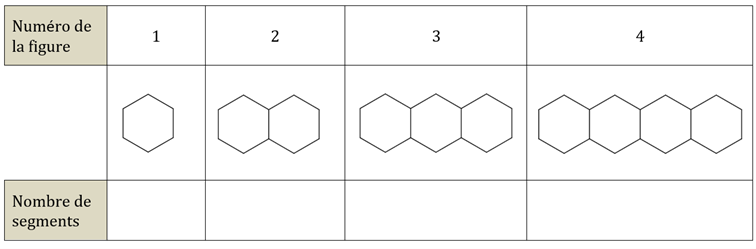
\includegraphics{img/suite.png}
	\begin{enumerate}
		\item \emph{(Sur cette feuille)} Complète le tableau.
		\item Combien de segments constitueront la figure n°5 ?
		\item Quelle est la formule qui lie le numéro de la figure (\(n\)) au nombre de segments (\(s\)) ?
		\item De combien de segments sera constituée la figure n°10 ?
		\item Quel est le numéro de la figure constituée de 56 segments?
	\end{enumerate}
